\chapter{Contributions}

In the following sections, we present the main contributions related to the Train Benchmark framework.

\section{A Real-life Model}

For our purpose to analyze graph queries, we use a model of train schedules provided by the \textit{Network Rail} company that runs, maintains, and develops Britain's rail tracks~\cite{network_rail}. Network Rail publishes a number of different data available to developers, some of them are the following:
\begin{itemize}
	\item{Real-time train positioning and movement event data}
	\item{Performance of trains against the timetable, measured as the percentage of trains arriving at their destination on-time}
	\item{Daily extracts and updates of train schedules}
\end{itemize}

The most adequate data for our aim is the daily schedules of trains, hence, the performance analysis is also based on this data.

\subsection{An Overview of the Train Schedules Data}\label{sec:schedules_overview}
The data of schedules can be divided into three different types of records\footnote{In the data of schedules a record actually represents a JSON object.} that are defined hereunder~\cite{schedules_data}:
\begin{itemize}
	\item{\textit{Association records}}: indicate the relationships between trains.
	\item{\textit{Schedule records}}: refer to the train schedules themselves.
	\item{\textit{Tiploc records}}: include information about timing point locations in the schedules.
\end{itemize}

At first, note that the trains themselves do not appear in a distinguished type of record, with the exception of their identifiers (\textit{Train UID}) that can be found in the association and schedule records, therefore, the data lacks of any information that describes the attributes of the physical trains.

An association is interpreted between two distinct trains that are somehow interconnected belonging to the same and only one location. For example, a dividing association means that a train separates into an other one in a particular station~\footnote{From now on, we use the words location and station as synonyms.}. However, an association does not necessarily occur, since there are trains that are not associated to any. To summarize, an association record always belong to the distinct trains, and one location.

A schedule record attaches locations to a certain train, thus, it defines a path of locations, which are divided into three different groups in a schedule, representing their positions in the path such as \textit{origin}, \textit{intermediate}, or \textit{terminating} location. One schedule always belongs to one train, even though a train can be referred by more schedules as well, and obviously, more than one schedule can include the same location.

Finally, \textit{Tiploc records} contain the locations.

\subsubsection{Cardinalities}

The data of schedules in Network Rail typically contain daily representations of the trains, however, an entire data model is available as well that contains every schedule information for each day. Since it includes a significantly larger data, from now on, we rely on this in our benchmark framework.

In the entire data, the cardinalities belonging to the individual types are depicted in Figure 1. %todo create a pie chart of cardinalities per entities
As can be observed, schedules represent the majority of the records, furthermore, only a small set of trains\footnote{Since train records are not defined in the data, in this case the number of trains are equal to the number of distinct train identifiers.} are in any kind of association with another train. The cardinality of locations indicates the number of unique locations, instead of their cumulated appearances. Regarding the latter, approximately 5.8 million number of locations occur as destinations attached to the schedules. It leads to the fact that the average number of attached destinations to a schedule is $15.66$.

\subsection{Mapping to a Model}\label{sec:mapping_schedule}

The previously introduced data of train schedules must be transformed to a graph on which the measurements can be accomplished. The corresponding domain derived from the data is depicted in Figure 2. %todo add a mesmerizing metamodel, or ER diagram and some footnote:this is actualy represented in blah blah to clarify blah blah
%todo don't mix the concepts of graph and metamodel, or domain and model, use a consistent expression
By mapping the domain to a graph leads to four different types of vertices: \textsf{Association}, \textsf{Station}, \textsf{Schedule}, and \textsf{Train}. The station symbolizes the location, and the references---such as \textsf{association}, \textsf{associative}, \textsf{destinations}, and so on---follow the same approaches introduced in Section \ref{sec:schedules_overview}, and they are mapped to directed edges in the graph. 

One newly introduced edge is the \textsf{neighbor} connection among the stations. The presence of a \textsf{neighbor} edge between two stations implicates the existence of a path from the first station to the second via the same schedule, and these stations follow each other in the schedule's destinations. In other words, the consecutive stations from a schedule's path become adjacent. Figure 3 demonstrates an example which nodes of stations are connected via \textsf{neighbor} edges, assuming that originally those locations belonged to the same schedule. As a conclusion, \textsf{Station1} and \textsf{Station2} are connected since they are adjacent in the destinations of \textsf{Schedule1}, on the contrary, \textsf{Station1} and \textsf{Station3} are not drawn to each other, since they are not consecutive stations among the schedule's destinations, despite the fact that both of them can be found in it. %todo draw a graph
Important to note that more than one adjacency in different schedules's stations do not implicate more \textsf{network} edges between the nodes.

\subsubsection{Attributes}

As can be observed in Figure 2, %todo add pic reference
there are different attributes belong to the vertices that can be found in the original data set as well. These attributes are briefly introduced below:
\begin{itemize}
	\item{\textsf{Schedule Planning}}: It can be \textit{Short-term}, or \textit{Permanent}.
	\item{\textsf{Status}}: It indicates the train status, and its possible value comes from the following enumeration: \textit{Freight}, \textit{Passenger}, \textit{Ship}, \textit{Bus}, and \textit{Trip}. Since a schedule can be a short-term overlay, thus, a temporary schedule may belong to a substitute bus or ship.
	\item{\textsf{Days}}: A seven-character binary variable, the first represents Monday, and last one is Sunday. For example, the attribute for a schedule---that runs on every Monday and Sunday---is equal to \textit{1000001}.
	%todo stpindicator is missing yet
	\item{\textsf{Start Date}}: The start date of the schedule.
	\item{\textsf{End Date}} : The end date of the schedule.
	\item{\textsf{UID}}: The unique train identifier.
	\item{\textsf{Category}}: Refers to the association's category that can be \textit{Divide}, \textit{Join}, \textit{Next}.
\end{itemize}
%todo mark that attributes with bold which will be used in the queries


\subsection{Model Analysis}\label{sec:model_analysis}
cardinalities
	prob distr
	scale-free, power-law dist
	random schedule factor -> important?





\section{Elaborate Analysis in Train Benchmark}

Our goal is to extend the Train Benchmark framework in order to analyze the performance of graph queries with a comprehensive model characterization, and to explore the performance and workload correlations via different descriptive metrics. The extensions are presented in the following sections.

\subsection{Workflows}

A workflow in the Train Benchmark is divided into different phases that are considered as the atomic execution units. An arbitrary chain can be created among the phases, which---during benchmarking---are executed consecutively. The following sections introduce an overview of the original and the extended workflow of the Train Benchmark.

\subsubsection{Original Workflow}
The workflow of the original framework is illustrated in Figure \ref{fig:old_train_workflow}. As it can be observed, the first phase is responsible for loading the model and query specification to memory. This implies that the definition of a query is immutable during the measurements. The second phase, \textsf{Check} symbolizes the validation, thus the query evaluation. Optionally, a validation can be followed by a graph transformation phase which modifies a subset of the elements. Finally, by simulating incremental validation, another \textsf{Check} phase follows, and the ensemble of transformations and revalidations is executed iteratively.


\begin{figure}[!ht]
	\centering
	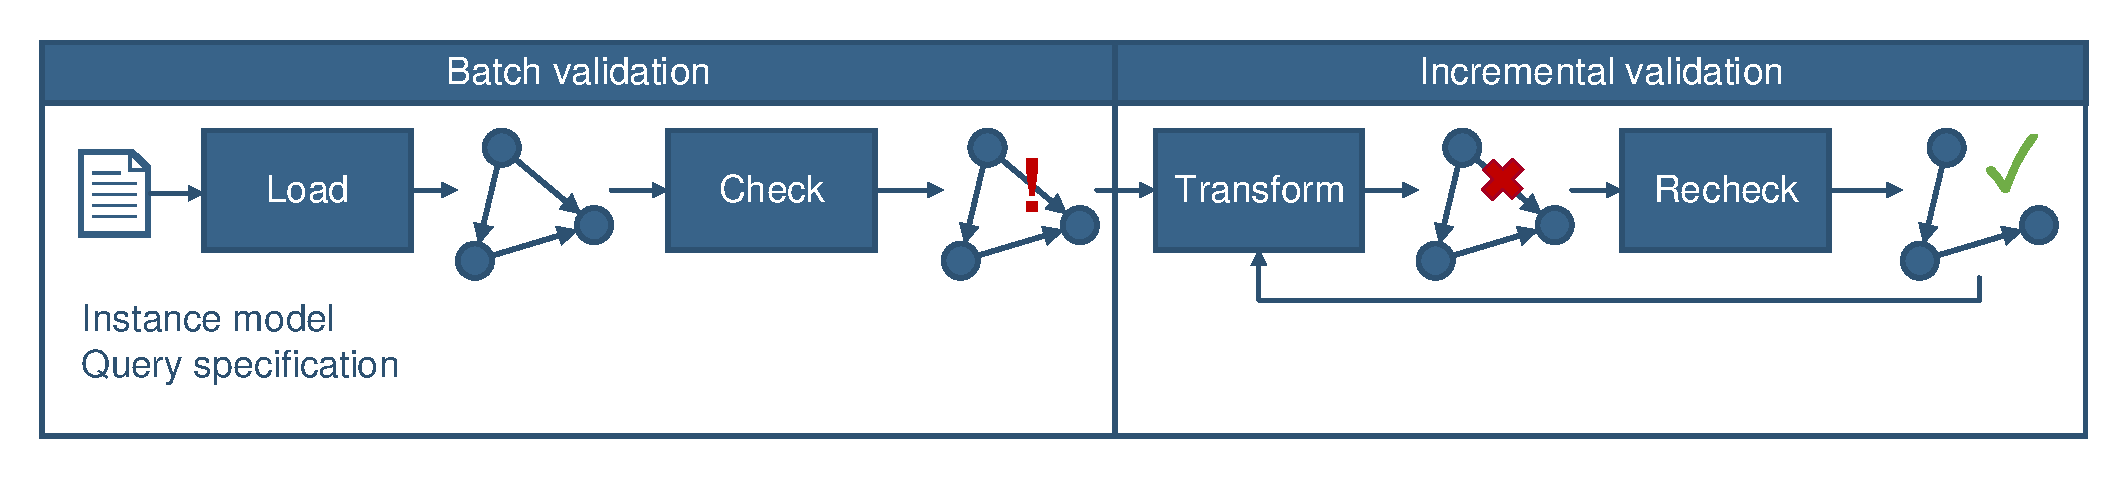
\includegraphics[width=150mm, keepaspectratio]{figures/trainbenchmark-sequence.pdf}
	\caption{The original workflow of Train Benchmark.}
	\label{fig:old_train_workflow}
\end{figure}

\subsubsection{Extended Workflow}\label{sec:extended_workflow}

The extended workflow of the Train Benchmark is depicted in Figure \ref{fig:new_train_workflow}. First, it is important to emphasize that the transformation and validation phases are omitted, meaning that this benchmark does not consider model modifications or model validations.

After loading the model, the framework calculates the model related metrics. Due to the fact that in the current phase of our research we do not consider model transformations, therefore, a particular model's metrics can be calculated only once in the beginning of the workflow, and more importantly, different runs of the benchmark can utilize the previously calculated metrics that belong to the same model. The solution is achieved by using a cache for the calculated metrics, and reusing its content if possible.

The features in the \textsf{Initialize} and \textsf{Build Query} phases are strongly correlated. As we already mentioned, a single run of the original benchmark evaluated only one immutable query, and thus, the dynamic replacement of its definition was not feasible in runtime. The absence of this feature is solved in the these two phases, since they entail the creation of dynamic queries. The first one provides a default query definition that can be parameterized, and the second phase assembles a complete query for the evaluation, as it injects parameters, or alters the entire syntax. The latter operation implies that entirely different queries can be executed in a sequence.

\begin{figure}[!ht]
	\centering
	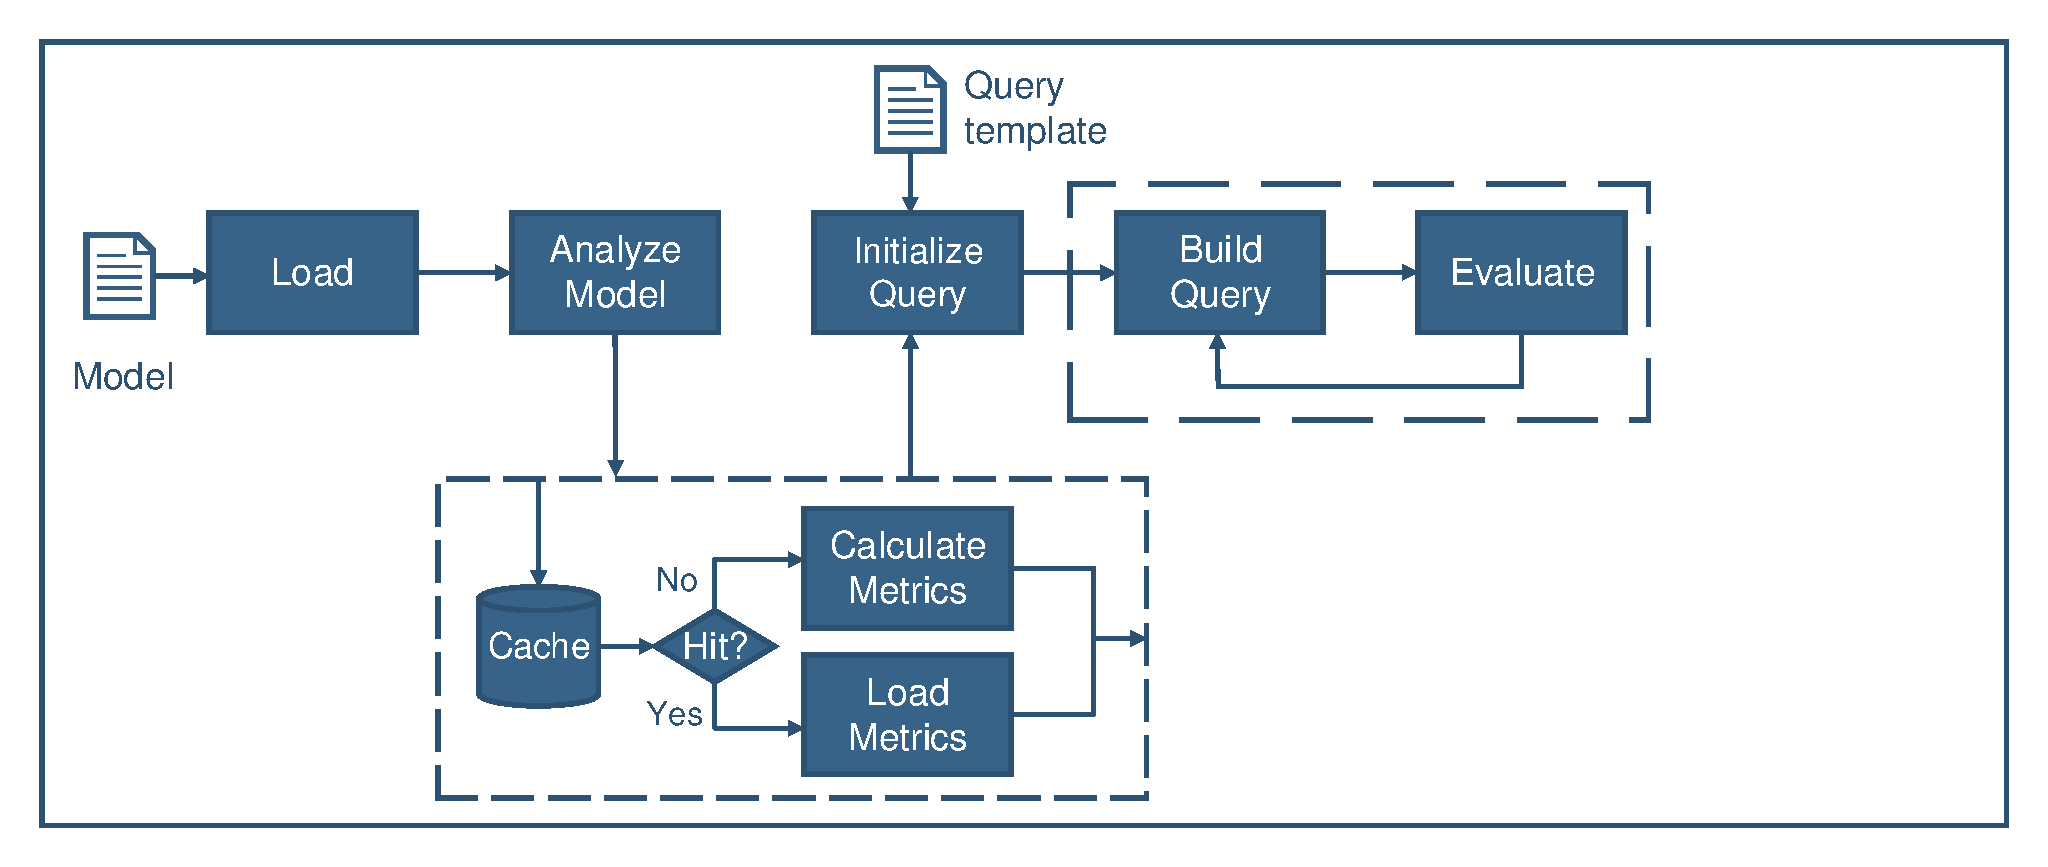
\includegraphics[width=150mm, keepaspectratio]{figures/workflow.pdf}
	\caption{The extended workflow of Train Benchmark.}
	\label{fig:new_train_workflow}
\end{figure}

The query analysis occurs before the evaluations, and according to the fact that the query definitions are mutable in run time, the query based metrics have to be calculated in every iteration. Lastly, the queries are executed in the last phase, and optionally, the building, calculating, and evaluating phases can be repeated.

\subsection{Metrics Calculation}
The new framework proposes two types of metrics. The first is the set of model descriptive metrics, and the second relates to the query syntaxes. 

\subsubsection{Model Metrics}
The model-based metrics are connected to graph metrics, and their naming convention also follows the commonly used metric names from graph theory. Since we are concentrating on RDF based tools in our research, we also define the corresponding interpretations of these metrics relating to RDF where it is necessary. The metrics are listed below.
%todo rdf and graph metrics
\begin{enumerate}
	\item{\textbf{Nodes}}: The number of nodes in the graph, or the number of subjects and objects in the RDF data.
	\item{\textbf{Edges}}: It is equal to the number of edges in the graph. Regarding RDF, this metric is considered as the number of predicates\footnote{With the consideration of \textit{rdf:type} predicates, the number of edges metric represents the number of triples.} in the data.
	\item{\textbf{Maximum Degree}}: The maximum number of predicates per subjects.
	\item{\textbf{Average Degree}}: It is determined by calculating the degree of every existing node.
	\item{\textbf{Average Degree Distribution}}: It denotes the probability that a randomly selected node’s degree is equal to the average degree.
	\item{\textbf{Higher Degree Distribution}}: The cumulative distribution of those nodes that have higher degrees than the average.
	\item{\textbf{Average Clustering Coefficient}}: This metric implies the calculation of clustering coefficient per every node.
	\item{\textbf{Average Shortest Path Length}}: The calculation of this metric requires the most cost, hence, the framework searches a limited number (100) of shortest paths between randomly chosen vertices and calculates the average length of them.
	\item{\textbf{Maximum Betweenness Centrality}}: The value of this metric is determined by the shortest paths. We count the occurrences of every intermediate node in the paths---which is the betweenness centrality of the vertices---and normalize the values to the $[0,1]$ interval by dividing them with the number of visited nodes. Since the value of betweenness centrality is individual per nodes, we use the maximum of them.
\end{enumerate}

Besides these metrics, we also calculate the degree distributions and cardinalities of the models, although these metrics are not included in the analysis to find metric and performance relationships.

\subsubsection{Query Metrics}

The query metrics relate to the query definitions, hence, they do not characterize the size of the result set---gained by the query evaluation---or the performance of the particular query.

Regarding RDF, the \textit{SPARQL} query metrics are determined by the \textit{Apache Jena ARQ}~\cite{jena} package. \textit{ARQ} proposes a way for parsing a SPARQL query into an algebra expression or an object, and analyzes its syntax. Relying on this solution, we introduce the following query metrics in Train Benchmark:
\begin{enumerate}
	\item{\textbf{Navigations}}: Represents the number of navigations or triples in the query.
	\item{\textbf{Filters}}: It denotes the number of selection conditions.
	\item{\textbf{Variables:}} The metric is equal to the amount of distinct variables.
	\item{\textbf{Constants:}} It is determined by the number of occurrences of constants.
\end{enumerate}
\subsection{The Architecture}

As we already emphasized, our research partly deviates from the field that the Train Benchmark originally investigates, however, most of the components from the framework are adequate for our goal and can be utilized. Figure \ref{fig:architecture} depicts the main components from the extended version of Train Benchmark, additionally, it denotes that which component is ignored---meaning that our work does not rely on it---or entirely reused, and which one is extended with further features or newly created.

\begin{figure}[!ht]
	\centering
	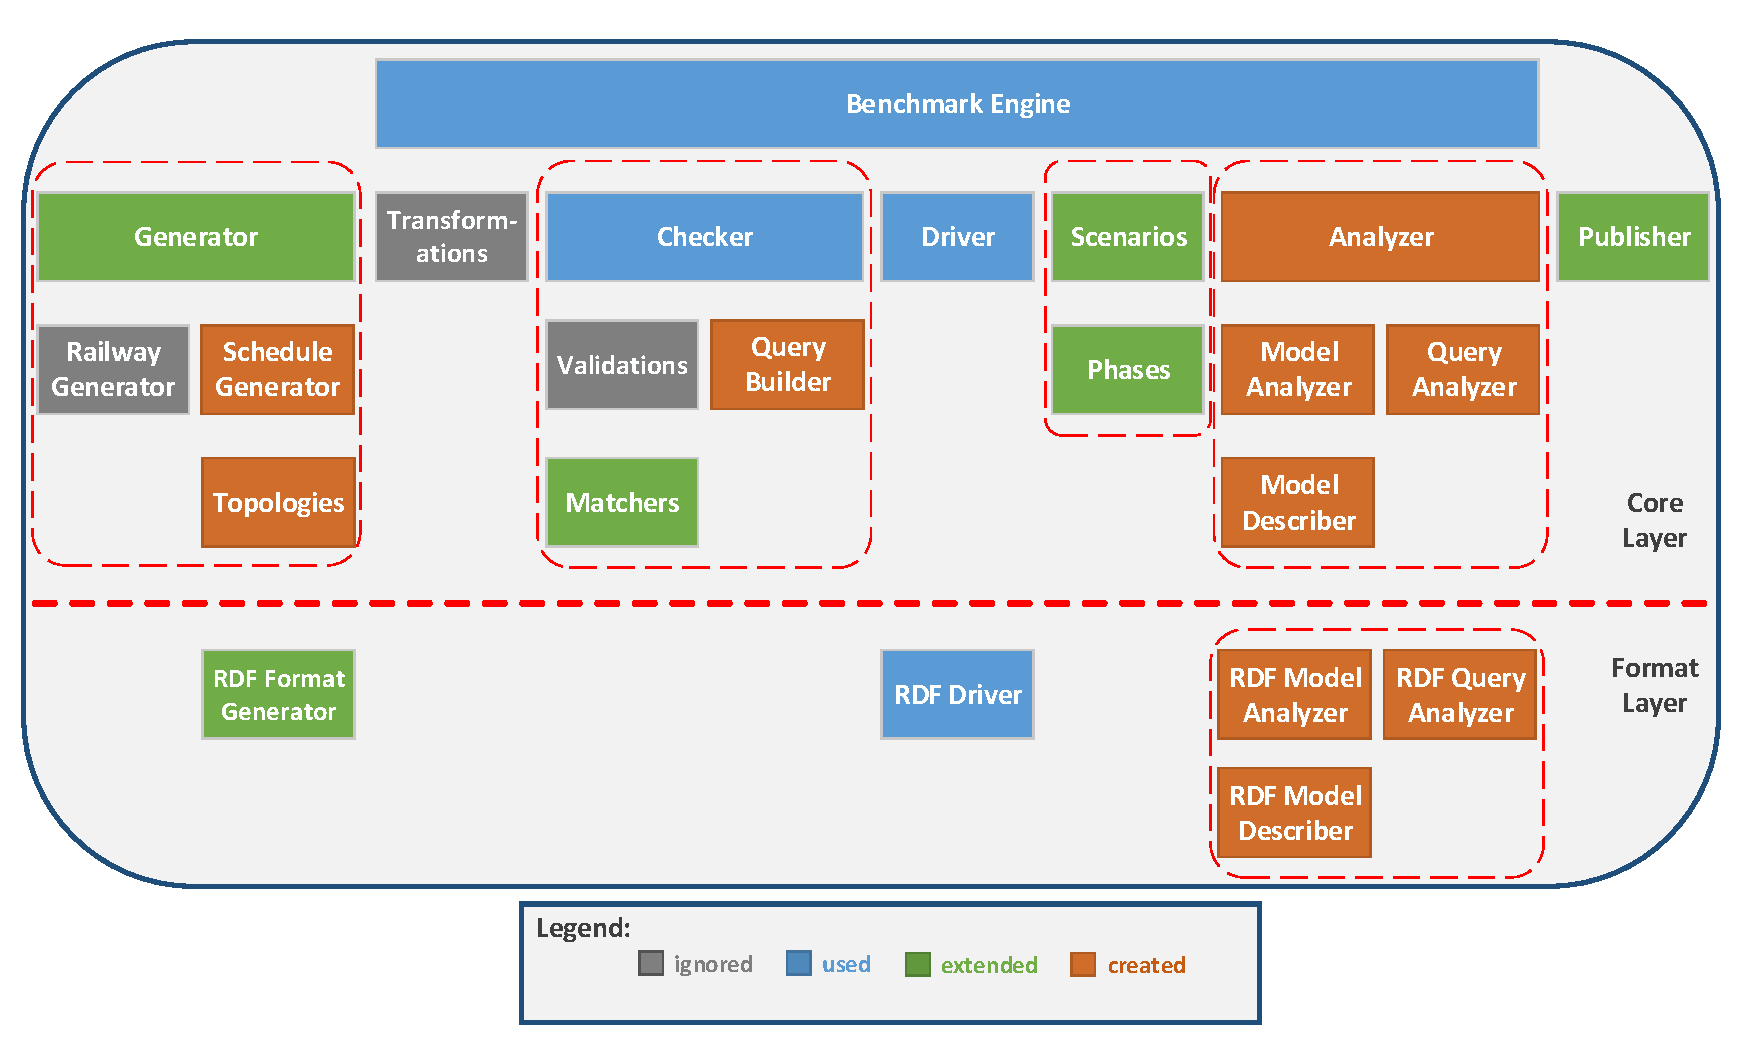
\includegraphics[width=150mm, keepaspectratio]{figures/architecture.pdf}
	\caption{The extended architecture of Train Benchmark.}
	\label{fig:architecture}
\end{figure}

In the following parts, we introduce the components and the related extensions.
\paragraph{Generators}
Originally, the measurements in the Train Benchmark framework were based on an artificially generated \textsf{Railway} model. The limitations of this model are already explored in Section \ref{sec:train}, and these observations entail the introduction of the \textsf{Schedules} model. \\%todo check reference later
The \textsf{Schedule Generator} component and the related \textsf{Topologies} are considered as new features in Train Benchmark, and the abstract \textsf{Generator} also had to be extended to support different domains in the framework.

\paragraph{Scenarios and Phases}

A \textsf{Scenario} represents a current workflow of phases. Our new scenario for analysis---so the extended workflow of the Train Benchmark---and the corresponding phases are described in Section \ref{sec:extended_workflow}. Actually, another newly created scenario belongs to the framework as well, which does not include query evaluations, and it only calculates the degree distributions and cardinalities of the models.

\paragraph{Benchmark Engine}
The \textsf{Engine} is responsible for evaluating a scenario and its phases consecutively.

\paragraph{Analyzer Components}

The ensemble of \textsf{Model} and \textsf{Query Analyzer} units became the new foundations of the framework. The \textsf{Model Describer} component includes the calculations of cardinality and degree distributions per models. Due to the fact that these metrics do not appear in the performance analysis, the component is separated.\\
The concrete calculations of metrics occur in the format related units such as the \textsf{RDF Model Analyzer}.

\paragraph{Driver}
The instances of the \textsf{Driver} interface manage the connection establishments between the databases and the framework. Furthermore, the loading of the models is also accomplished by the drivers.

\paragraph{Checker and Query Builder}

The query evaluations are achieved by the \textsf{Checker} component. Despite the fact that this unit originally executed model validations, yet, the component can be used for the evaluations.\\
Our new component, the \textsf{Query Builder} is responsible for creating and altering the query definitions in runtime.

\subsection{Regression Analysis}

\subsubsection{MARS}


\section{Model Generation}

The following sections represent the concepts of the new model generation elaborated in the Train Benchmark framework.

\subsection{Overall of the Generation Steps}
The new generation mechanism in Train Benchmark is based on the \textit{Schedule} model, introduced in Section \ref{sec:mapping_schedule}, and it consists of different steps which are depicted in Figure 1. %todo add generation steps figure
The necessary steps are described hereunder:
\begin{enumerate}
	\item The network among the stations is generated based on a graph topology.
	\item The generator creates schedule vertices and connects them to the stations, as they symbolize the destinations among the schedules.
	\item The generator instantiates the train nodes and attaches them to the schedules, as every schedule has a connection with a train.
	\item The attributes are initialized and linked to the nodes. The concrete values of the variables are determined the same distributions found in the original data.
	\item A connectivity inspection is executed on the graph.
	\item Finally, the model can be persisted to the particular format. %todo maybe can delete this, formats and tools are not emphasized
\end{enumerate}

\subsection{Topologies}
The most flexible part in the artificially generated models is the network among the stations, as using various well-known graph topologies. As we already emphasized, we generate the following networks:
\begin{itemize}
	\item Random Graph
	\item Watts-Strogatz Model
	\item Scale-free Networks of Barabási-Albert
	\item Hierarchical Network
\end{itemize}
The models and their algorithms are introduced in Section \ref{sec:topologies}, therefore, this section only includes the specific information about the .

\subsubsection{Random Graph}
From the two known algorithms, Gilbert's $G(n,p)$ model is adapted to the framework.

\subsubsection{Watts-Strogatz Model}\label{sec:watts_generation}

The commonly known generation algorithm is used with some extensions. Generally, the $N$ value in the algorithm---that represents the number of consecutive connected nodes---is a constant, which indicates a liner relationship between the number of edges and nodes, since every vertex has $N$ degree. However, we extend the algorithm by defining an inclusive lower ($N_1$) and upper ($N_2$) bound for $N$, as $N\in[N_1, N_2]$, and also assign a probability to $N$ that determines the number of consecutive interconnected nodes to be $N_1$ or $N_2$. As a result, this conducts to a generation that can obtain a more flexible, non-linear relationship between the number of edges and nodes.

\subsubsection{Scale-free Networks of Barabási-Albert}

In the original generation algorithm, every new vertex becomes to be connected to a constant number of disjunct nodes. Similarly to the notion in the Watts-Strogatz model generation (\ref{sec:watts_generation}), this constant value is converted to a random variable by a particular probability.

\subsubsection{Hierarchical Network}\label{sec:hierarcical_contribution}

The first difference between our constructed hierarchical graph and the original concept is that the former structure can be configured arbitrarily, since it is feasible to create $K_n$ complete subgraphs with optional $n$, instead of $K_5$. %todo use this notation in background too

The second most essential difference is the termination of the generation algorithm. As a general rule, the goal in Train Benchmark is that to generate arbitrary size of models by creating a precise number of nodes. Since the generation of hierarchical network is recursive instead of being incremental---as in the case of the three other topologies---it is inevitable to determine a termination from the recursion. The termination point is evident, as soon as the number of created nodes reaches the limit, the algorithm has to be stopped. However, it cannot be predicted in which phase the algorithm stops exactly. As a consequence, the possible failures have to be managed.

\begin{figure}[!ht]
	\centering
	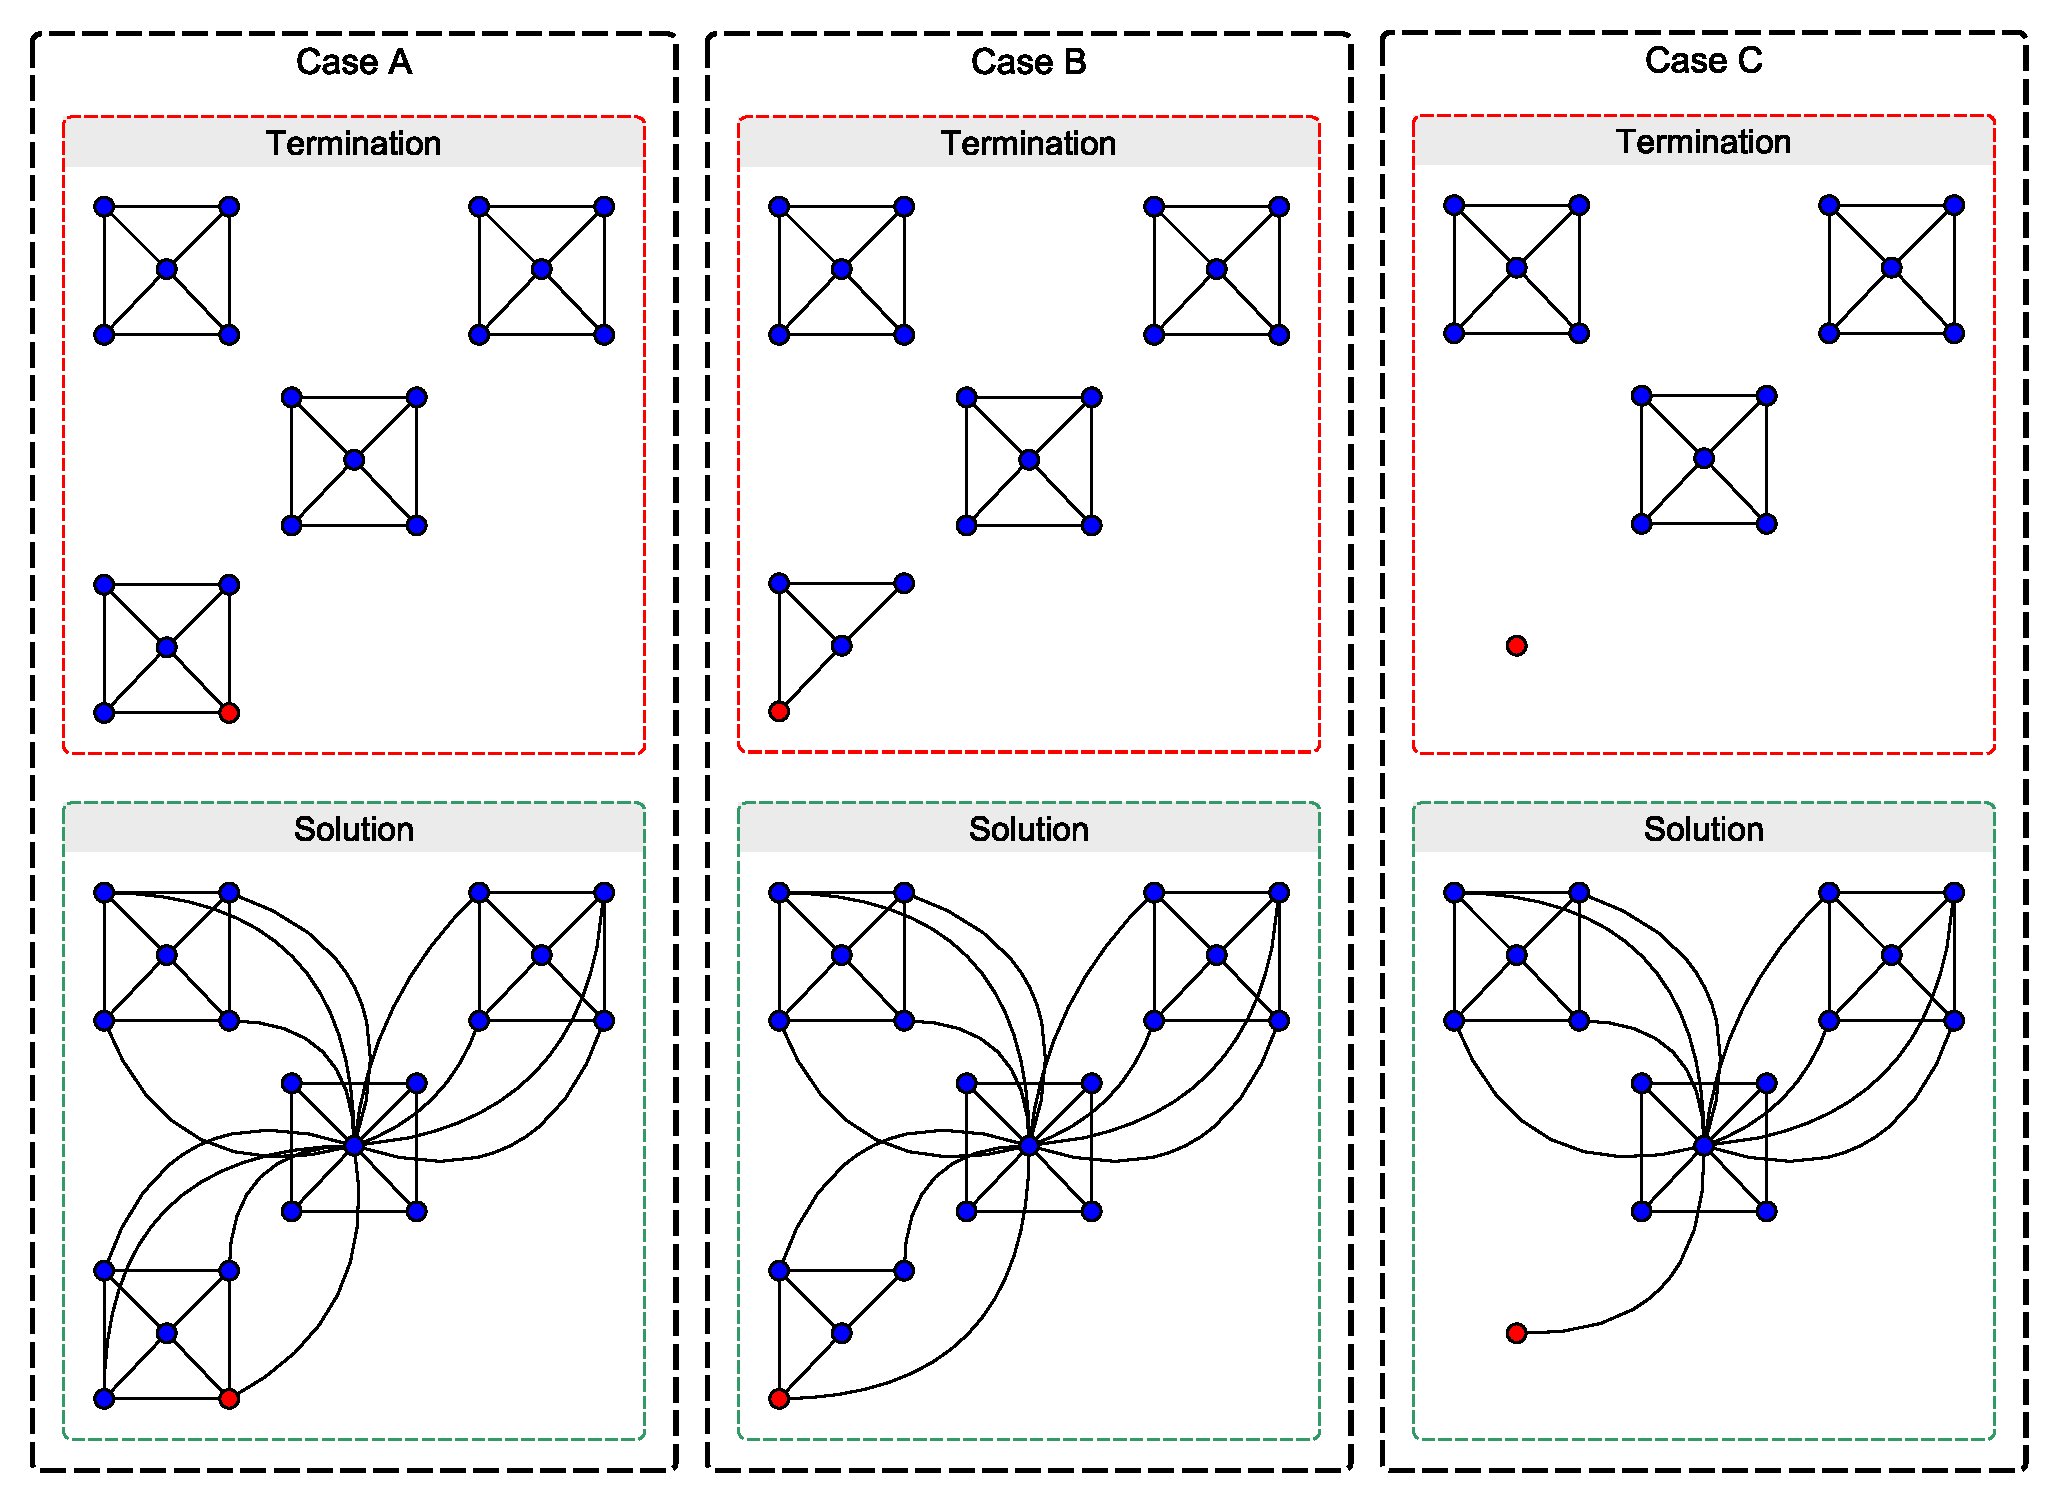
\includegraphics[width=150mm, keepaspectratio]{figures/hierarchical.pdf}
	\caption{Possible termination problems in the hierarchical graph generation}
	\label{fig:hierarchical_problems}
\end{figure}

The possible problematic cases are demonstrated in Figure \ref{fig:hierarchical_problems}. In \textsf{Case A}, \textsf{B}, and \textsf{C}, the expected numbers of nodes are 20, 19, and 16, respectively. As it can be observed in these cases, this limit is always reached before the fourth cloning occurs, since 5 clusters should be created with 25 vertices at the end of this step in the recursion.

In the solution in \textsf{Case A}, the generator stops the clone procedure and connects the diagonals to the center. Regarding \textsf{B}, the termination happens during the generation of a cluster. As a solution, the last cluster becomes partial, and similarly, every diagonal is attached to the center. \textsf{Case C} represents that scenario when the last cluster only consists of one node. To prevent isolation, the last vertex is considered as a diagonal, and be connected to the center.

\subsection{Schedule Connections}\label{sec:schedule_connections}

An important part of the generation is to connect the stations to schedules. As it was detected in Section \ref{sec:model_analysis}, the degree distribution of the schedule and station connections follows a power-law distribution. %todo add exponent value

In order to simulate a similar characteristic, we generate a power-law distribution from a uniform distribution\footnote{It is a more convenient way to use a uniform distribution which is easier to be accomplished due to a built-in random generator.} with the following formula~\cite{power_law_from_uniform}:
\begin{align}
	X = \Big[\big(x_1^{(n+1)} - x_0^{(n+1)}\big)y + x_0^{(n+1)}\Big]^{(\frac{1}{(n+1)})}
\end{align} 
where $n$ is the exponent or scale-factor, $y$ is a uniformly distributed variate on $[0,1]$, and $x_0$, $x_1$ are the minimum and maximum bounds of the interval. Finally, $X$ is determined for every schedule, and it represents the number of stations that have to be connected to the certain schedule. Due to this solution, the schedule and station connections show a power-law characteristic.

Another problem is choosing the appropriate stations. Actually, the value of $X$ is the length of the destinations path belonging to a schedule. As a result, for every schedule, the generator executes a \textit{breadth-first search} starts from a uniformly random station, and stops the algorithm as soon as it finds an $X$ length path. Finally, this path of stations is linked to the schedule.


\subsection{Possible Model Configuration}

In the artificially generated models, the cardinality, size, topology, and density is optionally configurable. 

Regarding cardinality, different proportions can be adjusted between the vertex types, as \textsf{Station}, \textsf{Schedule}, \textsf{Train}, and \textsf{Association}. The default adjustment is proportional to the observed cardinality in the case of the original data.

The size of the model---so the number of nodes---is calculated as $|V| = s \cdot 2^i$, where $s$ is the step size constant, $5000$ by default, and $i$ is a positive integer, given by the user.

As it was already emphasized, various graph topologies can be generated among the \textsf{Station} nodes, thus, the internal structure of the models and their degree distributions are also alterable. Moreover %todo finish

\subsection{Uniform Model Generation}

In the generation unit in Train Benchmark, it became possible to construct \textit{uniform} models with various topologies. Under the concept of uniformity, it is meant that the different models may consist of some particular \textit{static} subgraphs that are found in each one, furthermore, the models include the same number of nodes and edges, regarding the \textit{dynamic} parts, thus, the topologies as well.

%todo add a figure

\subsubsection{Static Subgraphs}
Regarding the static parts, the ensemble of \textsf{Train} and \textsf{Association} types of vertices can be classified to this category. Obviously, if the cardinality configurations---the proportion of the elements---in the models are the same, than these types of nodes and their relationships are equal, since they are generated by the same algorithm.

In terms of the \textsf{Schedule} nodes, achieving a completely uniform subgraph between the schedules and stations is not feasible. At first, note that those stations that are linked to the schedules, are chosen via a breadth-first search algorithm, which implicates different paths of destinations for the schedules in each model depending on the topology among stations. As a result, a precise, uniform internal structure between the schedules and stations cannot be generated, however the average degree of a \textsf{Schedule} node---thus, the amount of corresponding destinations---is precisely configurable, since the degree distribution of schedules is determined forward by a power-law generator (introduced in Section \ref{sec:schedule_connections}), yet, this configuration entails a problem.

The problem is the maximum size of paths among stations, reached by the BFS algorithm. Even though the Scale-free, random, and Watts-Strogatz models can be considered as arbitrary connected graphs, which leads to the assumption that a path exists among any two nodes with an optional length. However, this statement cannot be claimed in the case of hierarchical networks. There always exists a path between two arbitrary nodes in a hierarchical graph via the \textit{center node}\footnote{It is actually the first created node in algorithm, and in the further steps every diagonal is linked to this vertex.}. However, the maximum depth in this path without revisiting the center node again, is bounded. It is easy to confirm, since the sub hierarchies are not connected explicitly to each other, expect the center node. As a consequence, the maximum length between two nodes---considering the best scenario---consists of $\frac{|V|}{2^i}$ nodes, where $i$ is the current iteration value of the recursive algorithm. Considering an average case, the maximum length is $\frac{|V|}{2 \cdot 2^i}$. According to this number, the maximum bound of the power-law generation function is adjusted.

Note that, by achieving uniformity among the models, as using a consistent degree distribution in schedules based on the hierarchical graph, the generated models loose some of their real-life characteristics that was observed it the original data.

\subsubsection{Number of Nodes}

The question of nodes equality per graphs is related to the \textit{dynamic} parts of the graph, thus, to the topologies among the stations.

The only one problem about generating a graph with a certain number of nodes is the recursive algorithm of the hierarchical graph. Nevertheless, we already showed in Section \ref{sec:hierarcical_contribution} that the recursion is terminated appropriately, and the resulting problems are managed.

As far as the other structures are concerned, the ensemble of random graph and the Watts-Strogatz model is constructed by initializing $|V| = N$ number of vertices at first, and subsequently, the algorithms determine which one of them become adjacent. In the scale-free model generator, the nodes are created incrementally until $|V| = N$. As a deduction, a precise number of nodes in these topologies can be obtained.

\subsubsection{Number of Edges}

The only one challenge of obtaining an equal number of edges among the models is related to \textit{dynamic} parts of the graphs, the topologies. As it was already emphasized, the random graph, Watts-Strogatz model, and scale-free network can be configured optionally, which conducts the fact that arbitrary number of edges can be generated, even the same amount for every topology. Actually, in these types of networks, the amount of nodes and edges are handled respectively.


We are not finished yet, since Equation \ref{eq:fi_formula} is equal to the number of a completely finished hierarchical network's edges, however, the generator in Train Benchmark creates partial hierarchical networks with a particular large set of nodes, therefore, it terminates the recursive algorithm before it is finished. As a conclusion, if our expected hierarchical graph we intend to generate is $H$, then
\begin{align}
	|E_H| = |E_{F_i}| \cdot \frac{|V_H|}{|V_{F_i}|}
\end{align}
where $\frac{|V_H|}{|V_{F_i}|} \leq 1$, and the iterator $i$ is calculated from the expected maximum number of nodes found in $H$, as follows
\begin{align}
	|H| = (c+1)^i * n  \longrightarrow  i = \frac{\lg\frac{|H|}{n}}{\lg(c+1)}
\end{align}
and then use the ceiling of $i$ in the generator.

